\section{Constraint Dynamics}

Figure~\ref{fig:fig06_state_evolution} summarizes the state-evolution and data-assimilation workflow. The workflow combines model-based prediction, observational updates, and uncertainty estimation within the effective PCS representation.

\begin{figure}[tb]
\centering
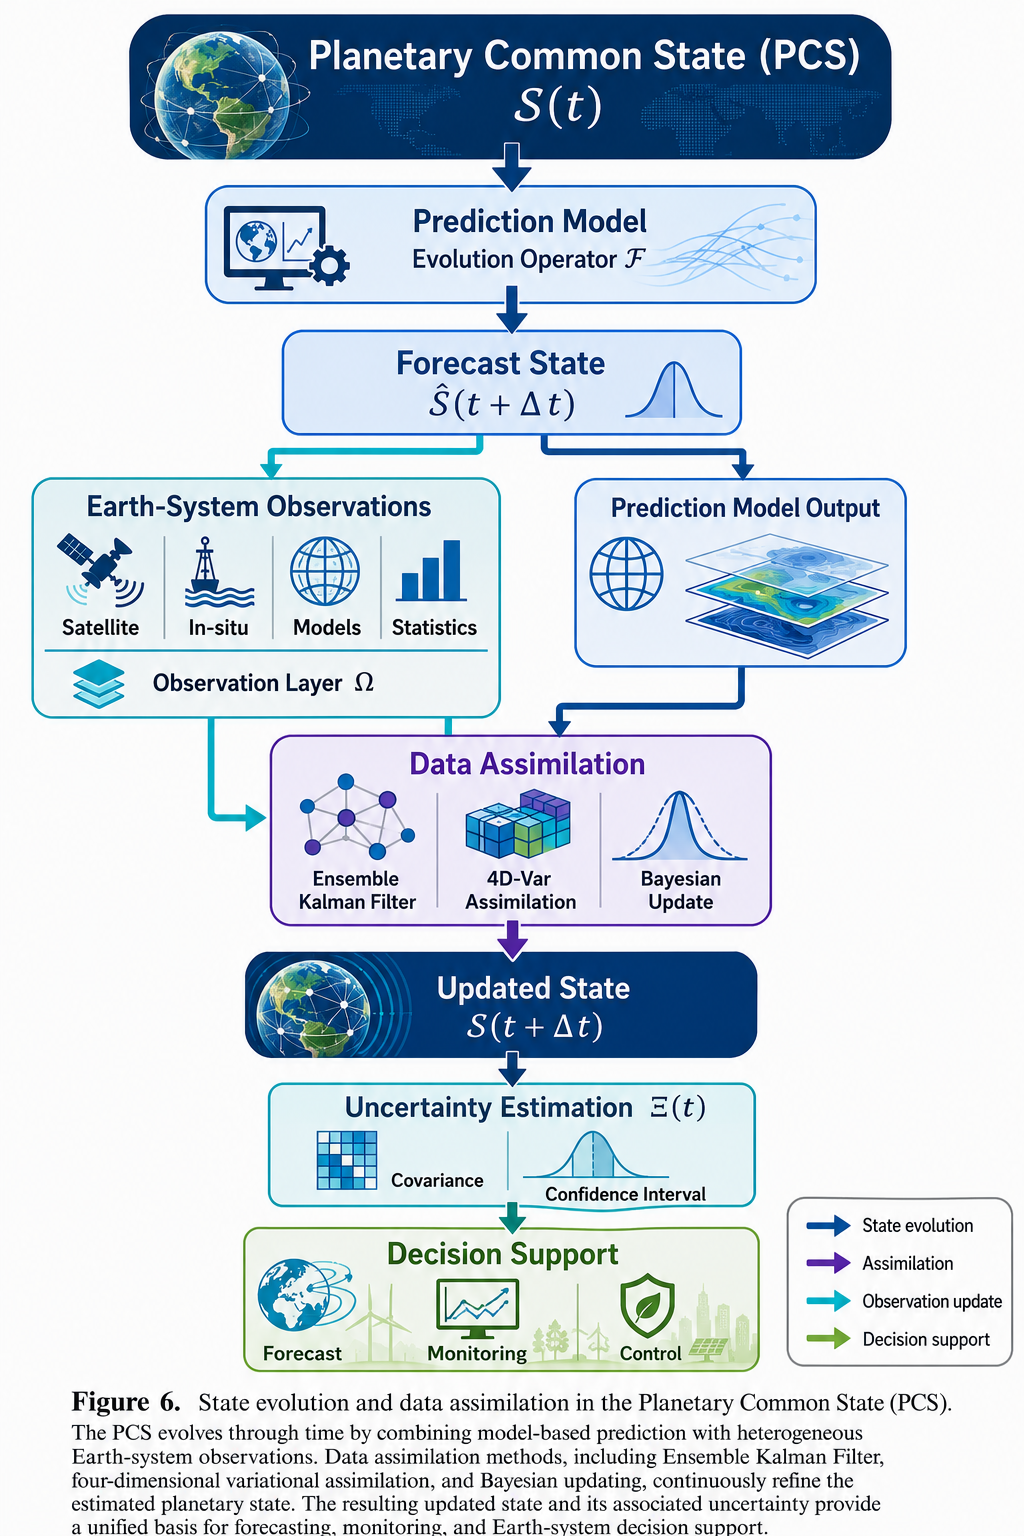
\includegraphics[width=\columnwidth]{figures/fig06_state_evolution.png}
\caption{State evolution and data assimilation in the Planetary Common State (PCS).}
\label{fig:fig06_state_evolution}
\end{figure}


\subsection{5.1 Evolution of the Constraint Operator}

The Unified Constraint Operator represents an instantaneous effective constraint state. Its macroscopic evolution may be written as

\[ \frac{D\mathbb{L}}{Dt}=\mathcal{F}(\mathbb{L},\Psi,t). \]

Here \(\Psi\) denotes the collection of relevant physical state variables and boundary conditions, and \(\mathcal{F}\) is an effective evolution operator to be inferred from data or constrained by domain models. It is not a microscopic law.

Remark 3 (Effective evolution). The variables collected in \(\Psi\) specify the resolved physical state, external conditions, and model inputs used for a particular application. The operator \(\mathcal{F}\) is therefore part of the macroscopic closure, and its domain and regularity assumptions must be stated whenever quantitative predictions are made.

\subsection{5.2 Constraint Sources}

The effective operator \(\mathcal{F}\) may receive contributions from thermal forcing, circulation, hydrology, chemistry, ecosystems, infrastructure, information flows, energy systems, and external boundary conditions. A schematic decomposition is

\[ \mathcal{F}=\sum_k \mathcal{F}_k. \]

This decomposition is an accounting convention. The terms \(\mathcal{F}_k\) must be defined through observables, models, or calibrated response functions.

\subsection{5.3 Stable Evolution}

Stable macroscopic evolution corresponds to slow change in the effective constraint state:

\[ \left\|\frac{D\mathbb{L}}{Dt}\right\|\ll 1 \]

after specifying the norm and time scale. Rapid growth of this norm is a diagnostic candidate for instability, not by itself proof of an imminent transition.

\subsection{5.4 Dynamic Equilibrium}

An approximately stationary constraint state satisfies

\[ \frac{D\mathbb{L}}{Dt}\approx 0. \]

This does not imply that physical processes cease. It indicates that the net projected constraint state is approximately stationary at the selected resolution.

This section introduces a macroscopic closure, not a microscopic equation of motion. Quantitative applications must define the norm, time scale, and data source used to estimate \(\mathcal{F}\).




\section{Constraint Coupling Theory}


\subsection{6.1 Coupling Matrix}

The projected components are generally coupled. When differentiability is justified, the effective coupling matrix may be written

\[ C_{ij}=\frac{\partial \pi_i(\mathbb{L})}{\partial \pi_j(\mathbb{L})}. \]

Equivalently, in projection coordinates, this can be represented locally as \(C_{ij}=\partial L_i/\partial L_j\). When differentiability is not justified, \(C_{ij}\) should be interpreted as an empirically estimated effective coupling coefficient.

Depending on the application, \(C_{ij}\) may be interpreted as an effective sensitivity, an effective response coefficient, or an empirical coupling estimate. The derivative notation is local and should not be read as an assumption of global differentiability. When the data support only finite perturbations or statistical dependence, the same symbol denotes the calibrated response measure used in that analysis.

\subsection{6.2 Empirical Estimation}

\(C_{ij}(t)\) may be estimated from lagged correlations \cite{Saltelli2008GSA}, response functions \cite{Saltelli2008GSA}, perturbation experiments, causal discovery methods, or data-assimilation sensitivity analysis \cite{Kalnay2003Assimilation}. The estimation method should be reported together with uncertainty, lag structure, and robustness checks.

\subsection{6.3 Physical Meaning}

Examples include thermal-flow coupling, flow-structural coupling, structural-informational coupling, and energy-viability coupling. These coefficients quantify effective cross-domain interaction. They do not introduce a new interaction beyond the mechanisms already represented in the underlying domain models.

Proposition 2 (Constraint coupling consistency). A coupling coefficient \(C_{ij}\) is interpretable only relative to a specified projection pair, normalization convention, time scale, and lag convention. Under these conditions, off-diagonal coefficients provide an effective representation of cross-domain sensitivity; without these conditions, comparisons among coefficients are not well-defined.

\subsection{6.4 Symmetric and Asymmetric Coupling}

In general, coupling need not be symmetric:

\[ C_{ij}\neq C_{ji}. \]

For example, a thermal anomaly may strongly affect ecological or hydrological projections, while the reverse influence may occur only indirectly or at longer time scales.

\subsection{6.5 Global Coupling Strength}

A simple aggregate measure of off-diagonal coupling is

\[ \Gamma=\sum_{i\neq j}|C_{ij}|. \]

The restriction \(i\neq j\) avoids including diagonal self-coupling unless explicitly stated. Large \(\Gamma\) indicates strong cross-domain coupling and may be associated with cascade risk, but the threshold for such risk must be empirically estimated.

Coupling coefficients are effective quantities whose interpretation depends on normalization, lag convention, and estimation method. They should not be treated as universal constants.




\section{Stability and Critical Transitions}


\subsection{7.1 Viability Functional}

Rather than defining stability solely as \(1-L\), UCT introduces a viability functional

\[ \mathcal{V}=\Phi(\mathbb{L}) \quad \text{or} \quad \mathcal{V}=\Phi(\mathbf{L}). \]

\(\mathcal{V}\) summarizes macroscopic persistence, adaptive capacity, or long-term stability as defined for the system under study. In the simplest linear approximation,

\[ \mathcal{V}\approx 1-L. \]

This approximation is useful only after \(L\) and its calibration have been specified.

Definition 7 (Viability functional). The map \(\Phi\) is an application-dependent functional from the operator or projection vector to a scalar measure of system viability. No universal form of \(\Phi\) is assumed. The approximation \(\mathcal{V}\approx 1-L\) is one possible low-dimensional closure, not a defining identity.

\subsection{7.2 Critical Threshold}

A scalar threshold \(L_c\), if used, is empirical and system-dependent. It should be estimated from historical transitions, controlled simulations, or independent validation datasets.

\[ L<L_c \quad \text{stable regime}, \qquad L\approx L_c \quad \text{transition region}, \qquad L>L_c \quad \text{post-threshold regime}. \]

These labels are diagnostic categories, not universal laws.

\subsection{7.3 Constraint Potential and Critical Surfaces}

In a multi-dimensional representation, critical behavior is more naturally associated with a surface or region in \(\mathbf{L}\)-space than with one scalar number. A potential landscape, if used, should be calibrated to the data and tested against alternatives.

\[ \mathcal{C}_{\mathrm{crit}}=\{\mathbf{L}: \Phi(\mathbf{L})=\Phi_c\}. \]

This expression defines an estimated critical surface in projection space; it does not imply a universal critical value.

\subsection{7.4 Early Warning Signals}

If UCT captures relevant slow modes near a transition, recovery time should increase as the system approaches the estimated critical surface \cite{Scheffer2009EarlyWarning,Dakos2008Slowing}. Other empirical signals may include increasing variance, rising autocorrelation, changing cross-domain coupling, and reduced adaptive capacity.

These are testable diagnostics. Their presence should be evaluated against null models and baseline indicators.

\subsection{7.5 Cascading Transitions}

A cascading transition occurs when perturbations propagate across projection domains through the coupling matrix. In this setting, a transition may be associated with increasing off-diagonal coupling,

\[ \Gamma\rightarrow\Gamma_c, \]

where \(\Gamma_c\) is an empirically estimated critical coupling level. No universal fixed value is implied.

This stability analysis identifies empirical diagnostics rather than universal thresholds. Critical surfaces, recovery times, and coupling thresholds must be estimated and compared with null models.


